\chapter{Étude numérique}
	\minitoc
	\section{Utilisation du code \textsc{GADGET-2}}

		Le code que nous utilisons pour faire évoluer notre système est
		\textsc{Gadget-2}~\footnote{récupérable sur
		\url{http://www.mpa-garching.mpg.de/gadget/}}~\cite{gadget2},
		écrit par Volker \textsc{Springel}. Seule une petite partie de
		ce qu'il fait nous intéresse : nous n'allons utiliser que les
		options concernant le \og~tree code~\fg. Toutes les autres
		options ne concernent que les simulations cosmologiques ou
		pourraient induire un comportement du code qui nous ferait
		perdre de la précision sur les calculs.

		Pour fonctionner, \textsc{Gadget-2} a besoin d'un fichier de
		configuration, dans lequel nous devrons jouer sur certains
		paramètres, et d'un fichier de conditions initiales respectant
		un format précis.

		\subsection{Fichier de conditions initiales}

			Le fichier de conditions initiales doit avoir le format suivant :
			\begin{enumerate}
				\item un en-tête contenant le nombre de particule de chaque type (~Gaz, Halo, Disque, Bulbe, Étoiles, Bndry~),
				la masse pour chaque type, divers autres informations utiles essentiellement aux simulations cosmologiques,
				\item les positions de chaque particules,
				\item leurs vitesses,
				\item un identifiant permettant de repérer chaque particule.
			\end{enumerate}
			Chaque bloc devant être encadré par sa taille en mémoire.

		\subsection{Fichier de configuration}

			Dans ce fichier, nous n'allons jouer que sur certains paramètres :
			\begin{itemize}
				\item \verb|OmegaLambda| : paramètre cosmologique représentant la densité d'énergie du
					vide, en le mettant à 0, nous faisons savoir à \textsc{Gadget-2} que nous ne faisons pas
					de simulation cosmologique.
				\item \verb|UnitLength_in_cm|, \verb|UnitMass_in_g| et \verb|UnitVelocity_in_cm_per_s|
					sont les unités dans lesquelles sont données, respectivement, les positions, masses et vitesses des particules en
					centimètre, gramme en centimètre par seconde. Ce sont ces facteurs de conversion
					qui donne l'unité de temps interne à \textsc{Gadget-2}. Nous utilisons
					les parsecs ($ 1 pc = 3.086 \times 10^{18} cm$) pour les positions, les kilogrammes
					($1 kg = 1000 g$) pour la masse, et les mètres par seconde ($ 1 m.s^{-1} = 10^2 cm.s^{-1}$)
					pour les vitesses. Ces unités nous donnent comme unité de temps
					interne :
					\begin{align}
						v &= \frac{d}{t} \notag \\
						t &= \frac{d}{v} \notag \\
						t &= \frac{3.086 \times 10^{18}}{10^2} = 3.086 \times 10^{16} s \notag \\
						t &= 9.77894 \times 10^8 ans
					\end{align}
				\item \verb|SofteningStarsMaxPhys| : paramètre de lissage de la force, permettant d'éviter
					qu'elle \og~n'explose~\fg~à cause d'une collision entre 2 particules trop proches.
					C'est sur ce paramètre qu'il faut jouer pour assurer la stabilité du système sur
					un grand nombre de temps dynamiques.
				\item \verb|ErrTolTheta| : représente l'angle d'ouverture, ou résolution angulaire, minimum.
					Celui-ci est fixé à $0.5$ et n'est plus modifié ensuite.
			\end{itemize}

		\subsection{Lissage de la force}

			Nous souhaitons nous placer dans la limite fluide afin
			de minimiser les effets de relaxations dû aux
			collisions à deux corps. Pour cela, nous pouvons jouer
			sur deux paramètres : le nombre de particules que nous
			mettons dans le système, et le paramètre de lissage.
			Étant limité en temps, nous ne pouvons pas lancer de
			simulations avec un très grand nombre de corps : les
			plus grosses simulations que nous lançons ont 100 000
			particules, et occasionnellement 500 000. Pour une
			évolution pendant 100 temps dynamiques, elles prennent
			environ 709 minutes en les faisant tourner sur 8 cœurs,
			et cela peut aller jusqu'à 1020 minutes.

			Le lissage est une borne, en distance, en deçà de laquelle nous considérons un potentiel minimum valant :
			\begin{align}
				\psi(r_{i} \sim 0) = - G \dfrac{m_i}{r_{i} + \epsilon}
			\end{align}
			où $r_i$ est le module de distance d'une particule
			numérotée $i$. $\epsilon$ est le paramètre de lissage
			de la force. Afin de nous placer dans la limite fluide,
			$\epsilon$ doit être tel qu'il contienne un nombre
			$N_\epsilon$ de particule grand devant 1 mais petit
			devant le nombre total de particule du système.
			Habituellement, c'est $N_\epsilon$ qui est choisi,
			imposant ainsi $\epsilon$, mais nous avons choisi
			$\epsilon$ imposant ainsi $N_\epsilon$.

		%	Dans un amas, la densité est plus forte au centre que
		%	sur le bord. Les effets de relaxation sont donc plus
		%	important au centre, le $\epsilon$ doit y minimiser ces
		%	effets, même s'il n'a aucun effet sur les bords de
		%	l'amas.
			À cause d'instabilité, il est important de décrire la
			dynamique au centre de l'amas avec la meilleur
			précision possible. Il est donc nécessaire d'être dans
			la limite fluide au centre. Il est alors intéressant de
			le relier à la densité centrale, plutôt que d'utiliser
			une distance inter-particulaire moyenne. Nous
			définissons donc $\alpha$ tel que :
			\begin{align}
				\alpha = \dfrac{\rho(0)}{\rho_\mathrm{moy}} = \dfrac{\rho(0)}{M} \frac{4}{3} \pi R^3
			\end{align}
			avec $M$ la masse totale de l'amas, $R$ le rayon de
			l'amas, et $\rho(0)$ la densité centrale de l'amas. La
			densité d'un volume de taille $\epsilon$ et la densité
			de l'amas nous donne donc :
			\begin{align}
				\rho_\epsilon &= \alpha \rho_\mathrm{moy}					\notag \\
				N_\epsilon    &= \alpha \frac{4}{3} \pi \epsilon^3 \dfrac{3N}{4\pi R^3}	\notag \\
					      &= \alpha N \( \dfrac{\epsilon}{R} \)^{3}
			\end{align}
			$N$ étant le nombre total de particules de l'amas. $N$,
			$R$ et $\alpha$ étant fixés, nous sommes ainsi libres
			de choisir $N_\epsilon$ ou $\epsilon$ pour répondre à
			nos besoins.

	\section{Générateur de conditions initiales}

		Pour obtenir nos conditions initiales, qui devront suivre un
		profil de \textsc{King}, nous allons utiliser la méthode de
		réjection, l'une des plus facile à mettre en place. Nous allons
		tirer aléatoirement la position et la vitesse des particules
		dans une boîte, puis nous n'en garderons qu'une partie en
		utilisant la fonction de distribution comme densité de
		probabilité. Pour commencer, nous utilisons les limites de
		notre modèle pour restreindre nos tirages à une boîte de taille
		\mbox{$\left[ - r_{\mathrm{max}}; r_{\mathrm{max}} \right]$}
		pour les distances et \mbox{$\left[ -v_{\mathrm{max}};
		v_{\mathrm{max}}\right]$} pour les vitesses :

		\begin{itemize}
			\item vitesse maximum : l'énergie totale du système est bornée supérieurement par l'énergie de libération :
				\begin{align}
					E = \dfrac{1}{2} m v_i^2 + m\psi(r) &< E_l \notag \\
					E_l - m\psi(r) &> \dfrac{1}{2} m v_i^2 \notag \\
					v_\mathrm{max}^2 = 2\(\dfrac{E_l}{m} - \psi(r)\) &> v_i^2 \notag \\
					v_{\mathrm{max}} = \sqrt{2\(\dfrac{E_l}{m} - \psi(0)\)} > v_i &> - \sqrt{2\(\dfrac{E_l}{m} - \psi(0)\)} = - v_{\mathrm{max}}
				\end{align}
			\item distance maximum : cette distance est obtenue pour
				$m\psi(r_{\mathrm{max}}) = E_l$. Il nous faut donc connaître le potentiel.
		\end{itemize}

		Le potentiel n'ayant pas d'expression analytique, nous allons devoir réutiliser
		notre algorithme de résolution numérique utilisé dans les chapitres précédents pour
		modèliser un King.

		Il nous faut aussi pouvoir redimensionner les quantités obtenues. Pour cela, le
		programme récupère dans un fichier de configuration les dispersions de vitesse
		$\sigma_v^2$, rayon de c\oe ur $r_c$, temps de relaxation $T_c$ et distance au
		soleil $R_\odot$ dans les unités du catalogue de \textsc{Harris}. Toutes sont
		ensuite transformées en unités SI (~mètre, kilogramme, seconde~). Comme nous
		avons pu le voir dans le chapitre~\ref{King::Chapitre} traitant du modèle de
		King, la masse $m$ d'une particule n'influence pas le profil de densité final :
		\begin{align}
			r_c^2 &= \dfrac{\sigma^2}{4\pi G m \rho_0} \notag \\
			      &= \dfrac{(\sigma_v^2)^2 m}{8\pi G m \rho_0} \notag \\
			      &= \dfrac{(\sigma_v^2)^2}{8\pi G \rho_0} \notag \\
			\Rightarrow \rho_0 &= \dfrac{(\sigma_v^2)^2}{8\pi G r_c^2}
		\end{align}
		Pour redimensionner la densité, nous n'avons donc pas besoin de connaître la
		masse d'une particule. Ce constat nous permet de laisser ce paramètre libre et
		de jouer sur le nombre de particules dans le système. En effet, une fois la
		densité obtenue, nous pouvons l'intégrer sur le volume de l'amas pour trouver la
		masse totale de ce dernier, puis, connaissant le nombre de particules, en déduire
		la masse d'une étoile par la relation :
		\begin{align}
			m = \dfrac{M_{tot}}{\text{Nombre de particules}}
		\end{align}
		Déduire le reste des paramètres utiles pour le redimensionnement est ensuite
		assez simple.
		La distance maximum $r_{\mathrm{max}}$ est déduite de la résolution
		numérique des équations.

		Pour pourvoir tout redimensionner, nous avons aussi besoin de connaître l'énergie
		de libération de l'amas. Pour cela, nous utilisons le théorème de \textsc{Gauss}
		et un petit raisonnement simple. Par définition, nous avons :
		\begin{align}
			E_\mathrm{min} < E < E_l < 0 \ &\text{ et } \ E_l = \frac{p^2}{2 m} + m \psi(r)
			\intertext{soit :}
			\psi(r) = \frac{1}{m}\(E_l - \frac{p^2}{2 m}\)
			\intertext{La valeur maximale du potentiel est donc atteinte pour $p = 0$ :}
			\psi_\mathrm{max} = \psi(R) = \frac{E_l}{m}
			\intertext{Hors du système, le théorème de \textsc{Gauss} nous dit qu'il peut être vu comme une particule ponctuelle de masse $M$. Le potentiel hors de l'amas s'écrit donc :}
			\psi(r) = -\frac{G M}{r}
			\intertext{Par continuité, nous avons :}
			\psi(R) = \frac{E_l}{m} = -\frac{G M}{R}
		\end{align}

		Pour générer des nombres aléatoires dans l'intervalle voulu, nous utilisons la
		fonction \verb|double ran2(long seed)| tiré de~\cite{NumericalRecipesC}, dont
		nous nous servont ainsi :
		\lstset{language=C, label=algo::tirage, frame=shadowbox}
		\begin{lstlisting}
			double  x  = rmax - 2.0 * rmax * ran2(seed),
				y  = rmax - 2.0 * rmax * ran2(seed),
				z  = rmax - 2.0 * rmax * ran2(seed),
				vx = vmax - 2.0 * vmax * ran2(seed),
				vy = vmax - 2.0 * vmax * ran2(seed),
				vz = vmax - 2.0 * vmax * ran2(seed);
		\end{lstlisting}
		Notre système étant sphérique, nous ne devons pas avoir de vitesse et de module
		de distance supérieurs, respectivement, à $v_{\mathrm{max}}$ et
		$r_{\mathrm{max}}$, de plus nous avons une probabilité
		\mbox{$f(E)/f(E_\mathrm{min})$}
		d'avoir une particule d'énergie $E$. Cette énergie minimale est l'énergie
		potentielle d'une particule au centre de l'amas, et de vitesse nulle.
		Une fois qu'une particule respecte ces conditions et que \og les probabilités sont
		avec elle \fg, nous l'enregistrons.

		Le programme écrit au fur et à mesure les coordonnées cartésiennes et vitesses
		des particules selectionnées dans un fichier dans les unités standards : mètre
		pour les distances et mètre par seconde pour les vitesses.

	\section{Vérification des résultats\label{Verif_gene}} %du générateur}

		Maintenant que nous avons un générateur de conditions initiales, il convient de
		le vérifier. C'est-à-dire d'utiliser les coordonnées, vitesses et masses des
		particules pour remonter à des quantités comme la densité ou l'énergie de
		l'objet créé, puis de comparer ces quantités aux prédictions théoriques.
		Notamment, nous avons généré un profil de King, qui se doit donc d'être au
		Viriel, mais aussi d'avoir une certaine pente sur la densité, comme vu dans les
		précédents chapitres.

		Pour faire les vérifications, nous avons choisi d'utiliser des histogrammes.

		\subsection{Masse et densité}

			\begin{wrapfigure}{l}{0.28\textwidth}
				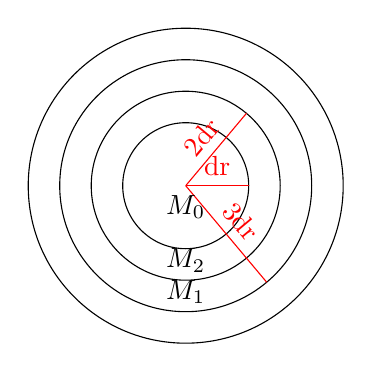
\begin{tikzpicture}[scale=0.8]
					\draw (2.5,2.5) circle(1);
					\draw (2.5,2.5) circle(1.5);
					\draw (2.5,2.5) circle(2);
					\draw (2.5,2.5) circle(2.5);
					\draw[red] (2.5,2.5) -- (3.5,2.5) node[midway, above] {$\mathrm{dr}$};
					\draw[red] (2.5,2.5) -- ++(50:1.5) node[sloped, above, midway] {$2 \mathrm{dr}$};
					\draw[red] (2.5,2.5) -- ++(-50:2) node[sloped, above, midway] {$3 \mathrm{dr}$};
					\draw (2.5,2.5) node[below]{$M_0$};
					\draw (2.5,1.15) node[below]{$M_1$};
					\draw (2.5,1.65) node[below]{$M_2$};
				\end{tikzpicture}
				\caption{Découpage de l'amas généré\label{schema::bin}}
			\end{wrapfigure}
			Le premier histogramme que nous générerons sera celui représentant
			la masse en fonction du rayon. Notre objet étant sphérique, nous allons le
			découper en intervalles de taille $\mathrm{dr}$ comme sur le schéma ci-contre. La fonction
			de masse représente la masse se trouvant dans l'intervalle \mbox{$\left[0; j \mathrm{dr}\right]$}.
			Pour la calculer, nous comptons le nombre de particules dans chaque chaque coquille sphérique de largeur $dr$ (~bin~), puis,
			après avoir multiplié par la masse d'un particule, nous sommons, pour le bin
			$j$, tous les bins inférieurs.

			En même temps que nous calculons la fonction de masse, nous pouvons calculer la
			densité en divisant la masse dans un bin par le volume du bin :
			\begin{align}
				\rho_\mathrm{bin} &= \dfrac{M_\mathrm{bin}}{V_\mathrm{bin}} \notag \\
				\rho_i = \rho\( (i+1) \mathrm{dr}\) &= \dfrac{M_{\mathrm{bin}\ i}}{V_{\mathrm{bin}\ i}} \\
					&= \dfrac{M_{\mathrm{bin}\ i}}{\frac{4}{3}\pi ( (i+1)\mathrm{dr})^3 - \frac{4}{3}\pi ( i\mathrm{dr})^3} \notag \\
					&= \dfrac{3 M_{\mathrm{bin}\ i}}{4 \pi \mathrm{dr}^3 \left[ (i+1)^3 - i^3\right]} \notag \\
					&= \dfrac{3 M_{\mathrm{bin}\ i}}{4 \pi \mathrm{dr}^3 \left[ 3 i^2 + 3 i + 1\right]} \\
					&= \dfrac{3 \(M_i - M_{i-1}\)}{4 \pi \mathrm{dr}^3 \left[ 3 i^2 + 3 i + 1\right]}
			\end{align}
			avec $M_{-1} = 0$.

			La densité obtenue et celle prévue par la résolution numérique sont très proche,
			comme le montre le graphique~\ref{Comp_gene-theo}.
			\begin{figure}[h!]
				\centering \includegraphics[scale=0.5]{graphe/Comp_dens_gene-theo_5000.pdf}
				\caption{Comparaison entre la résolution numérique et la densité donnée par le générateur\label{Comp_gene-theo}}
			\end{figure}

		\subsection{Énergie et potentiel}

			La partie la plus complexe de la vérification est le calcul de l'énergie. Deux
			choix s'offrent à nous :
			\begin{itemize}
				\item la méthode force brute : nous calculons l'énergie totale en utilisant
					l'expression newtonienne du potentiel :
					$$
						E_{tot} = \frac{1}{2}\sum_{i = 1}^{N} m_i v_i^2 - G \sum_{i = 1}^{N} \sum_{j < i} \dfrac{m_i m_j}{|| r_i - r_j ||}
					$$
					avec $N$ le nombre de particule Le problème de cette méthode est qu'elle nécessite $N^2$
				opérations et n'est donc pas intéressante lorsque nous travaillons avec un grand
				nombre de particules. De plus, si deux particules sont très proche,
				l'énergie potentielle va diverger.
				\item la réflexion : nous avons déjà calculé la densité, et nous avons
					la fonction de masse, nous avons tout ce qu'il nous faut pour
					avoir le potentiel à partir de l'équation de \textsc{Poisson}.
			\end{itemize}

			Nous allons calculer le potentiel en résolvant l'équation de \textsc{Poisson}. Voyons
			comment la résoudre avec ce que nous avons.
			\begin{align}
				\Delta\psi &= \frac{1}{r^2}\dfrac{d}{dr}\( r^2 \dfrac{d \psi(r)}{dr} \) = 4\pi G \rho(r) \notag \\
				r^2 \dfrac{d \psi(r)}{dr} &= 4\pi G \int_0^r \rho(r) r^2 dr = G M(r) \notag \\
				\intertext{La densité est une fonction continue par morceau, nous pouvons donc écrire :}
				M(r)    &= 4\pi \int_0^r \rho(r) r^2 dr \notag \\
					&= 4\pi \sum_{j = 0}^{i - 1} \int_{j \mathrm{dr}}^{(j+1)\mathrm{dr}} \rho_j r^2 dr + 4\pi \int_{r_{i-1}}^r r^2 dr \text{, $r\in\left[ r_{i - 1}; r_i \right]$} \notag \\
					&= 4\pi \sum_{j = 0}^{i - 1} \rho_j \left[ \dfrac{r^3}{3} \right|_{j \mathrm{dr}}^{(j+1)\mathrm{dr}} + 4\pi\rho_i\left[\dfrac{r^3}{3}\right|_{r_{i - 1}}^{r} \notag \\
					&= 4\pi \sum_{j = 0}^{i - 1} \dfrac{\rho_j}{3} \mathrm{dr}^3 \( (j+1)^3 - j^3)\) + \dfrac{4\pi \rho_i}{3} \(r^3 - i^3\mathrm{dr}^3\) \notag \\
					&= M(r_{i-1}) + \dfrac{4\pi \rho_i}{3} \(r^3 - i^3\mathrm{dr}^3\) \notag \\
				\intertext{Ceci nous permet alors d'écrire le potentiel :}
				\psi(r) - \psi(0) &= G \int_0^r \dfrac{M(r)}{r^2} dr \notag \\
				\psi\(r_i\) - \psi(0) &= G \sum_{j = 0}^{i} \left\{\int_{j \mathrm{dr}}^{(j+1)\mathrm{dr}} \dfrac{M(r_{j-1})}{r^2} + \dfrac{4\pi \rho_j}{3 r^2} \(r^3 - j^3\mathrm{dr}^3\) dr\right\} \notag \\
				\intertext{avec $ r_i = (i+1) \mathrm{dr} $}
				\psi(r_i) - \psi(0) &= G \sum_{j = 0}^{i} \left\{M_{j-1} \left[ \dfrac{-1}{r}\right|_{j \mathrm{dr}}^{(j+1)\mathrm{dr}} + \dfrac{4\pi \rho_j}{3} \( \left[ \dfrac{r^2}{2} \right|_{j \mathrm{dr}}^{(j+1)\mathrm{dr}} - j^3\mathrm{dr}^3 \left[ \dfrac{-1}{r}\right|_{j \mathrm{dr}}^{(j+1)\mathrm{dr}} \)\right\} \notag \\
						    &=  G \sum_{j = 0}^{i} \left\{\dfrac{1}{j ( j + 1 ) \mathrm{dr}} \( M_{j - 1} - \dfrac{4\pi \rho_j}{3}j^3\mathrm{dr}^3 \) + \dfrac{4\pi \rho_j}{6}\( 2 j + 1 \)\mathrm{dr}^2\right\}
				\intertext{Pour le bin central $j = 0$, nous avons :}
				\psi(dr) - \psi(0)  &=  G \dfrac{4\pi \rho_0}{6}\mathrm{dr}^2
			\end{align}

			Pour obtenir la constante $\psi(0)$, nous allons nous servir des conditions sur le bord du système. En effet, nous avons vu plus haut que :
			\begin{align}
				\psi_\mathrm{max} = \psi(R) &= - \frac{G M}{R} \\
				\intertext{Donc :}
				\psi(R) + \psi(0) - \psi(0) &= - \frac{G M}{R} \\
				\psi(0) &= - \frac{G M}{R} - \(\psi(R) - \psi(0)\) \\
				\psi(0) &= \frac{E_l}{m} - \(\psi(R) - \psi(0)\)
			\end{align}

			Le graphique~\ref{potentiel_5000} nous montre le potentiel théorique et le potentiel calculé par cette méthode.

			\begin{figure}[h!]
				\centering \includegraphics{graphe/Potentiel_ci-100000.pdf}
				\caption{Comparaison entre la résolution numérique et le potentiel donné par le générateur\label{potentiel_5000}}
			\end{figure}

		\subsection{Forme de l'amas}

			Maintenant que la densité et le potentiel de l'amas
			généré ont été vérifiés, il faut aussi vérifier que
			l'amas ne change pas de forme : nous générons un amas
			sphérique, nous devons~\footnote{il a en effet été
			montré qu'un \textsc{King} non collisionnel est
			stable~\cite{JPerez96}} conserver un amas sphérique
			après l'avoir fait évoluer. Pour vérifier que la forme
			de l'amas ne change pas, nous allons regarder comment
			évoluent les axes principaux d'inertie. Pour ce faire,
			nous allons calculer les valeurs propres de la matrice
			d'inertie :
			\begin{align}
				\mathfrak{I} &= \(\begin{array}{ccc}
							\int \(y^2 + z^2\) dm & - \int xy dm & - \int xz dm \\
							-\int xy dm & \int \(x^2 + z^2\) dm & - \int yz dm \\
							-\int xz dm & -\int yz dm & \int \(x^2 + y^2\) dm
						\end{array}\) \\
					     &= \(\begin{array}{ccc}
							A & - D & - E \\
							-D & B & - F \\
							-E & -F & C
						\end{array}\)\notag
				\intertext{L'équation aux valeurs propres va alors s'écrire :}
				\left|\mathfrak{I} - \lambda \mathbb{I}\right|  &= \(A - \lambda\)\left[\(B-\lambda\)\( C-\lambda\) - F^2\right] + D \(-D\(C-\lambda\) - F E\) - E \left[ D F + E\(B - \lambda\)\right] \notag %\\
			\end{align}
			polynôme d'ordre 3 que l'on résout avec la méthode de \textsc{Cardan}.

			Une fois ces valeurs propres obtenues, si elles
			existent, nous traçons l'évolution des rapports
			$\lambda_1 / \lambda_2$ et $\lambda_3 / \lambda_2$, les
			valeurs propres étant numérotées dans l'ordre
			décroissant \mbox{$\lambda_1 > \lambda_2 > \lambda_3$}.

	\section{Résultat des simulations}
		Les seules simulations que nous avons pu faire dans le cadre du stage sont des tests pour vérifier la stabilité de nos conditions initiales, ce qui représente déjà un travail important.

Nous avons donc commencé par générer des amas comportant un faible nombre de particules (~1000 ou 5000 particules~) afin de vérifier notre générateur, ce sont les résultats montrés par la courbe~\ref{Comp_gene-theo} pour 5000 particules, puis~\ref{potentiel_5000} pour 100000 particules.
Il nous faut maintenant vérifier que ces amas restent stables sur un grand nombre de temps dynamiques. Les simulations présentées dans cette section utilisent un amas réel dont les données ont été récupéré dans le catalogue de
\textsc{Harris} et à partir du travail fait dans les chapitres précédents. Il s'agit de l'amas NGC 288. Pour cet amas, les calculs analytiques donnent $\alpha = 439.72$.

Passons maintenant à l'étude de la stabilité sur le "long" terme de nos amas. Nous montrerons ici les résultats des tests
décrits dans la section~\ref{Verif_gene}.

Dans la table~\ref{eps_Neps}, nous avons indiqué quelles valeurs de $\epsilon$ nous avons utilisées : la valeur de $N_\epsilon$ correspondante, le nombre de particules qui sont au-delà du rayon des conditions initiales de l'objet,
et quelques autres informations utiles pour trouver la valeur qui nous intéresse.
	\begin{table}[h!]
		\begin{center}
			\begin{tabular}{|c|c|c|c|c|c|}
				\hline
				\multirow{2}{1cm}{$\epsilon\ \(pc\)$}	&	\multirow{2}{1cm}{$N_\epsilon$}	&	\multirow{2}{1cm}{$N_\mathrm{out}$}	&	\multirow{2}{3.5cm}{Fraction d'énergie cinétique emportée}	&	\multirow{2}{3.5cm}{Fraction d'énergie potentielle emportée}	&	\multirow{2}{2cm}{Courbes associées} \\
					&	&	&	&	&	\\
				\hline
				\hline
				$0.0194028$	&	$ 0.44 $		&	380	&	$ 0.00013573$			&	$ 0.00081092$	&	\ref{soft::0.019}, \ref{soft::0.019-Ax}\\
				\hline
				$0.05$		&	$ 7.52 $		&	239	&	$ 8.04628\times 10^{-5}$	&	$ 0.000488421$	&	\ref{soft::0.05}, \ref{soft::0.05-Ax}\\
				\hline
				$0.15$		&	$ 203.17 $		&	282	&	$ 9.91201\times 10^{-5}$	&	$ 0.00106241$	&	\ref{soft::0.15}, \ref{soft::0.15-Ax}\\
				\hline
				$0.20$		&	$ 481.58 $		&	653	&	$ 0.000265688$			&	$ 0.00265207$	&	\ref{soft::0.2}, \ref{soft::0.2-Ax}\\
				\hline
				$0.30$		&	$ 1625.34 $		&	919	&	$ 0.000433181$			&	$ 0.00466071$	&	\ref{soft::0.3}, \ref{soft::0.3-Ax}\\
				\hline
			\end{tabular}
		\end{center}
		\caption{Valeurs testés pour $\epsilon$ et $N_\epsilon$\label{eps_Neps}}
	\end{table}

	Discutons maintenant les résultats.

	\begin{description}
	%\paragraph{$\epsilon = 0.0194028$ :}
	\item[$\epsilon = 0.0194028$]
	Ce paramètre donne des résultats satisfaisants : sa densité évolue assez peu sur le temps de la simulation comparé aux valeur de $\epsilon > 0.05$, et ses axes d'inertie restent constant
	(~le bruit visible sur les graphes est dû au bruit statistique, bruit statistique dû au nombre fini de particules~). Par contre, le nombre de particules dans un volume de taille $\epsilon$ est trop petit : nous sommes trop loin de la limite fluide.

	%\paragraph{$\epsilon = 0.05$ :}
	\item[$\epsilon = 0.05$]
	Les fractions d'énergie potentielle et cinétique emportées par les particules sortantes sont minimum pour ce paramètre. De plus, sa densité et ses axes d'inertie évoluent peu, comme pour la valeur précédente.
	Cette fois, nous avons suffisamment de particules dans le volume de taille $\epsilon$.

\begin{figure}[h!]
	\centering \includegraphics[scale=0.5]{graphe/Comp_dens_gene-theo_0-05.pdf}
	\caption{Comparaison entre la densité numérique et la densité après évolution : $\epsilon = 0.05$\label{soft::0.05}}
\end{figure}

\begin{figure}[h!]
	\centering \includegraphics[scale=0.5]{graphe/Axial_ratio_0-05.pdf}
	\caption{Évolution des rapports des axes d'inertie : $\epsilon = 0.05$\label{soft::0.05-Ax}}
\end{figure}

	%\paragraph{$\epsilon = 0.15$ :}
	\item[$\epsilon = 0.15$]
	Pour ce paramètre, la fraction d'énergie potentielle emportée est de l'ordre de $0.1\%$, ce qui représente un changement important pour le rapport du Viriel $2 E_c/E_p$
	(~avec $E_c$ l'énergie cinétique et $E_p$ l'énergie potentielle~) : le profil de densité a complétement changé, l'amas s'est étendu.
	Par contre, il commence à se passer des choses intéressantes au niveau des axes d'inertie : pendant une grande partie de la simulation l'amas conserve sa forme, puis une instabilité arrive et il se déforme. % selon
%	l'un des axes, mais reste constant sur le second.
	\item[$\epsilon > 0.15$]
	Les valeurs supérieurs de $\epsilon$ ne sont alors clairement pas intéressante. De plus, ces valeurs sont trop proches du rayon de cœur de l'amas qui est de l'ordre de $10^{16}\ m = 0.32\ pc$ : en lissant toute
	la partie centrale de l'amas, nous changeons sa dynamique. En effet, il suffit de voir que, en augmentant le paramètre de lissage, l'instabilité menant à une déformation arrive de plus en plus tôt.
	Les déformations deviennent plus violentes.
	\end{description}

	La valeur de lissage optimale se trouve donc entre $\epsilon = 0.05$ et $\epsilon = 0.15$, pour une dizaine de particule (~pour $N_\epsilon = 10$, $\epsilon \sim 0.05497\ pc$~).





\chapter{Comparaison entre Gadget et un code Vlasov\label{Chap::VlasovGadget}}
	\minitoc%

	% \todo[inline]{Ce chapitre en est à peine à son premier jet. Toutes les figures ne sont pas encore commenté (ça arrivera dans le courant de la
	% semaine). Il manque aussi les figures contenant tous les $j$ sommé.}

	% Une des questions qui se posent avec notre approche concerne sa validité. En effet, à quel point gadget peut il
	% être proche d'un programme résolvant directement les équations de Vlasov-Poisson. Dans ce chapitre, nous tentons
	% d'apporter des éléments de réponse.

	% Avant de présenter les résultats obtenus à propos de notre instabilité, nous allons présenter un travail que nous avons effectué en parallèle
	Dans ce chapitre, je vais présenter un travail de comparaison de la mesure de la fonction de distribution dans l'espace des phases et du profil de densité
	entre le code $N$-corps \textsc{Gadget-2} et un code résolvant
	numériquement l'équation de Vlasov pour un système sphérique. Ce projet a été réalisé dans le cadre d'une collaboration avec Stéphane
	Colombi, Sébastien Peirani, Thierry Sousbie et Yasushi Suto (\citet{C2PSS}, plus loin C2PSS). Après une description du code Vlasov dans la première section, 
	les résultats de mon travail seront présentés dans la section~\ref{Sec::VlaGad::Res}. 
	Ils correspondent à une étude préliminaire dont les conclusions nous ont conduit à écrire un article sur le sujet, dont je résumerai les résultats
	principaux dans la discussion de la section~\ref{Sec::VlaGad::Art}.

	Pour que nos comparaisons aient un sens, il faut que le système préserve au mieux sa symétrie sphérique car nous utilisons \textsc{Gadget-2} tel quel,
	notamment sans modification du calcul de la force qui imposerait par exemple qu'elle soit purement radiale. La sphère de Hénon, introduite dans la
	section~\ref{Chap::Anal::HénonSec}, représente dans ce cadre un excellent cas test car elle est sujette à une évolution dynamique non triviale et il a été
	prouvé dans de nombreuses études qu'elle est très peu sensible numériquement aux formes d'instabilités qui conduiraient à des déviations par rapport à la
	symétrie sphérique, telles que l'instabilité d'orbite radiale (voir par exemple~\citet{albada,roy,barneslanzel}). Nous effectuerons nos analyses pour deux
	types de conditions initiales: un cas \og{}chaud\fg correspondant à un rapport du Viriel $\gamma=-0.5$ et un cas \og{}froid\fg correspondant à
	$\gamma=-0.1$.
	
	% Pour comparer nos simulations, nous regarderons la correspondance entre l'espace des phases $(r, v_r)$ pour $j=0,425$, l'espace
	% des phases intégré sur $j$ et le profil de densité de l'objet. Nous effectuerons ces comparaison à différents temps afin
	% de montrer que nous obtenons bien le même comportement au cours de l'évolution du système. La simulation \textsc{gadget-2} utilisée ici comporte $10^6$
	% particules. L'article associé étudie aussi l'évolution de simulations composées de $10^5$ et $10^7$ particules.

	% Tous les diagrammes de l'espace des phases que nous allons étudier présenterons à gauche la simulation Vlasov et à droite la simulation
	% \textsc{gadget-2}, sauf si contre indication. Tous utilisent la même échelle de couleurs pour une même simulation. Le système d'unité utilisé
	% est le même que~\citet{1983PASJ...35..547F}.

	\section{Description du code Vlasov}

		% Nous considérons un système à symétrie sphérique.
	Le solveur de Vlasov que nous utiliserons dans ce travail sera désigné par \textsc{Vlasolve}. Il a été écrit par Thierry Sousbie en se basant sur l'article
	de~\citet{1983PASJ...35..547F}. Il est 
		présenté en détail dans~\citet{C2PSS} et j'en résume ici le principe.

		L'équation de Vlasov en symétrie sphérique s'écrit:
		\begin{align}
			\pderivn{f}{t} + v_r\pderivn{f}{r} + \(\dfrac{j^2}{r^3} - \dfrac{M(r)}{r^2}\)\pderivn{f}{v_r} = 0\label{Eq::ValGad::Pois}
		\end{align}
		avec $f = f(r, v_r, j, t)$ la fonction de distribution dans l'espace des phases du système au temps $t$, $r$ la position radiale, $v_r$
		la vitesse radiale et $j$ le moment angulaire. La fonction $M(r)$ donne la masse contenue à l'intérieur de la sphère de rayon $r$. Dans cette
		équation, et comme il le sera fait dans tous le reste de ce chapitre, nous avons choisi les unités telles que la constante gravitationnelle vaut $G=1$.

		Pour résoudre l'équation, l'espace des phases est discrétisé sur un maillage tridimensionnel de dimensions $\(N_r, N_v, N_j\)$ et tel que $(r, v_r,
		j)\in\(\left[r_\mathrm{min}; r_\mathrm{max}\right], \left[-v_r^\mathrm{max}; v_r^\mathrm{max}\right], \left[0;
		j_\mathrm{max}\right]\)$ avec $r$ évoluant logarithmiquement, $v_r$ linéairement et chaque tranche $k$ de $j$ telle que $j=j_\mathrm{max}\(k-1/2\)^2 / N_j^2$.
		
		Pour suivre numériquement l'évolution de $f(r, v_r, j, t)$, un schéma dit de \og{}splitting\fg est utilisé, inspiré d'un article de référence
		de~\citet{1976JCoPh..22..330C}. Dans ce schéma, chaque point $i$ du maillage est considéré comme une particule virtuelle. Pour calculer
		$f(r, v_r, j, t+\Delta t)$ en ce point, on remonte la trajectoire de cette particule virtuelle d'un pas de temps en arrière en séparant
		l'équation~\refeq{Eq::ValGad::Pois} en deux opérateurs:
		\begin{itemize}
			\item un premier opérateur permet d'obtenir la trajectoire balistique d'une particule, incluant la partie inertielle:
				\begin{align*}
					\pderivn{f}{t} + v_r\pderivn{f}{r} + \dfrac{j^2}{r^3}\pderivn{f}{u} = 0
				\end{align*}
			\item un second permettant de calculer l'accélération gravitationnelle:
				\begin{align*}
					\pderivn{f}{t} - \dfrac{M(r)}{r^2}\pderivn{f}{v_r} = 0
				\end{align*}
		\end{itemize}
		Ces deux opérateurs, alliés à un schéma de type \og\sm\fg, permettent d'obtenir la position de la particule virtuelle correspondant à chaque
		point du maillage au pas de temps précédent.
		La densité dans l'espace des phases est mesurée en ce point par interpolation sur la grille en utilisant des splines d'ordre 3.
		Elle est alors affectée au point $i$ de la grille au temps $t+\Delta t$ par application directe du théorème de Liouville.

		Notons que chaque tranche de moment angulaire $j$ peut être traitée séparément étant donné que le moment angulaire est un invariant du système.

		% L'axe selon $r$ évoluant logarithmiquement, un problème va se poser lorsque $r\to0$. Pour l'éviter, nous faisons l'approximation que
		% les particules à l'intérieur du rayon $r_\mathrm{min}$ sont libres. Ce rayon doit donc être suffisamment petit pour que cette approximation
		% soit vérifiée, mais suffisamment grand pour éviter la divergence du logarithme.
		% toutes les particules passant sous ce rayon $r_\mathrm{min}$ puissent évoluer comme des particules libres.

		Cette méthode ne permet de suivre qu'une fonction de distribution suffisamment lisse, notamment à cause de l'interpolation utilisée.
		Comme nous allons le voir, les variations des vitesses orbitales des différentes composantes du système induisent la filamentation de $f$ dans le sous-espace $(r,
		v_r)$.
		La résolution finie de la grille ne permet pas de suivre tous les détails de cette filamentation à petite échelle,
		et va donc naturellement les lisser par effet de diffusion, ou parfois malheureusement les amplifier par effet de crénelage. Nous verrons que ce
		dernier a peu d'impact sur la dynamique. Cependant, pour tenir compte des éléments dont nous venons de discuter, nous apodiserons la sphère de Hénon,
		supposée de masse totale unité, de la manière suivante:
		\begin{align*}
			g(r) = \mathrm{erf}\( \dfrac{R - r }{ r_\epsilon }\) + 1
		\end{align*}
		avec $R$, le rayon de l'objet choisi égal à $2$ et $r_\epsilon=0.5$. Pour corriger des effets de cette apodisation, la masse totale est renormalisée
		a posteriori. Cette apodisation sera bien entendu appliquée également aux conditions initiales des simulations $N$-corps.



		% Dans les sections suivantes, nous allons comparer ces deux codes en utilisant deux rapports du viriel: $\gamma=-0,5$ et $\gamma=-0,1$.
		% l'évolution de la sphère de Hénon avec un viriel de $\gamma=-0,5$ puis nous
		% enchaînerons sur une comparaison utilisant un viriel de $\gamma=-0.1$.

	\section{Comparaison entre les simulations Vlasov et \textsc{Gadget-2}}

	Dans cette section, nous discutons des comparaisons détaillées de \textsc{Gadget-2} et \textsc{Vlasolve} que nous réalisons pour des rapports du viriel $\gamma=-0.5$ et
	$\gamma=-0.1$. Étant donné le choix des unités (masse totale du système unité, taille initiale $R=2$), on peut donc s'attendre à ce que le système plus froid ($\gamma=-0.1$)
	évolue dynamiquement plus vite que l'autre système comme argumenté par exemple dans~\citet{1983PASJ...35..547F}. Par conséquent, les analyses ont été réalisées en des
	temps plus petits pour $\gamma=-0.1$ que pour $\gamma=-0.5$.
	% et que nous supposons que la constante gravitationnelle
	% est égale à $G=1$.

	Pour conduire les comparaisons, les simulations \textsc{Vlasolve} réalisées ont une grille de résolution 
	$\(N_r, N_v, N_j\) = \(1024, 1024, 512\)$ et un pas de temps $\Delta t=5\times 10^{-4}$. Les simulations \textsc{Gadget-2}, quant à elles, composées de $10^6$ particules,
	utilisent un paramètre de lissage de la force $\epsilon=10^{-3}$ et un pas de temps maximum de $\Delta t = 0.1$.\footnote{Sachant que le temps dynamique initiale est de l'ordre de $2\pi$.}
	Les autres paramètres de \textsc{Gadget-2} sont
	ceux par défaut, notamment l'angle d'ouverture $\theta=0.5$ et la tolérance sur l'erreur {\tt ErrTolForceAcc} $= 0.005$ pour le calcul de la force.

	\subsection{Tests préliminaires: sphéricité et isotropie dans les simulations $N$-corps}
	% Nous avons voulu comparer les résultats donnés par  (écrit par Thierry Sousbie en se basant sur~\cite{1983PASJ...35..547F}) et le
	% code $N$-corps \textsc{gadget-2}.

	% Tous les diagrammes de l'espace des phases que nous allons étudier présenterons à gauche la simulation Vlasov et à droite la simulation
	% \textsc{gadget-2}, sauf si contre indication. Tous utilisent la même échelle de couleurs pour une même simulation. Le système d'unité utilisé
	% est le même que~\citet{1983PASJ...35..547F}.

		Comme mentionné dans l'introduction de ce chapitre, la sphère de Hénon est connue pour préserver la symétrie sphérique. L'hypothèse de la
		sphéricité étant un élément fondamental de nos analyses, nous allons donc vérifier sa validité dans nos simulations $N$-corps. Cela est fait dans les
		figures~\ref{Fig::VlaGad::SpheTest::AR} et~\ref{Fig::VlaGad::SpheTest::AR0.1} pour $\gamma=-0.5$ et $\gamma=-0.1$, respectivement. En accord avec les
		résultats de la littérature, les rapports des valeurs propres du tenseur d'inertie restent très proches de $1$ avec un écart maximum
		de l'ordre du pourcent pour $\gamma=-0.5$ et de $3\%$ pour $\gamma=-0.1$.

		L'analyse des propriétés d'ellipticité du système peut être complétée par la
		mesure de l'anisotropie dans l'espace des vitesses $\beta$. En effet, cette dernière, si elle est trop prononcée, peut être la source d'instabilités
		d'orbites
		radiales (voir la section~\ref{Chap::Sec::ROI}). Nos conditions initiales imposent $\beta=0$. La figure~\ref{Fig::VlaGad::SpheTest::Aniso} montre que pour
		$\gamma=-0.5$, $\beta$ reste très proche de $0$ et donc que le caractère isotropique du système dans l'espace des vitesses est presque parfaitement
		préservé. En revanche, pour $\gamma=-0.1$ (figure~\ref{Fig::VlaGad::SpheTest::Aniso0.1}), $\beta$ devient positif, plus particulièrement au moment
		du croisement des trajectoires ($t\sim 3$) puis son amplitude diminue et se stabilise à $\beta\simeq0.4$.
		Cela veut dire que la composante radiale des vitesses est significativement amplifiée par rapport à la composante tangentielle,
		mais les valeurs propres du tenseurs d'inertie ne montrent pas d'évolution significative. Le système ne développe donc pas d'instabilité d'orbites radiales
		essentiellement parce qu'il n'y a pas de germe sur laquelle elle pourrait se développer,
		% mais cette
		% amplification est insuffisante pour provoquer l'instabilité d'orbites radiales,
		comme attendu d'après les discussions de la
		section~\ref{Chap::Sec::ROI}.

		En conclusion, nous pouvons considérer que nos sphères de Hénon conservent suffisamment leur caractère sphérique pour pouvoir sans crainte effectuer
		des comparaisons de la structure fine de la fonction de distribution dans l'espace avec le solveur \textsc{Vlasolve}.

		% Avant de comparer ces deux codes, nous allons vérifier deux points. Le premier est l'effet du lissage de la force $\epsilon$ sur
		% l'évolution de la sphère de Hénon. Ensuite, nous vérifierons que les simulations \textsc{Gadget-2} conserve la sphéricité et
		% l'isotropie de l'objet.

			% La symétrie sphérique est imposée par le code Vlasov.
			% Nous allons donc vérifier que notre simulation conserve sa symétrie sphérique.
			% Dans le même temps, nous allons vérifier que le résultat de l'effondrement de la sphère de Hénon reste isotrope.

			% C'est ce que montrent les figures~\ref{Fig::VlaGad::SpheTest::AR} et~\ref{Fig::VlaGad::SpheTest::Aniso} pour $\gamma=-0,5$.
			% La première montre l'évolution des rapports d'axes au cours du temps. Ils restent tous deux très proches de $1$. La sphère de Hénon
			% reste bien sphérique tout du long de son évolution. La figure~\ref{Fig::VlaGad::SpheTest::Aniso} montre l'évolution de
			% l'anisotropie au cours du temps. Son évolution confirme que la sphère reste isotrope.

			% Les figures~\ref{Fig::VlaGad::SpheTest::AR0.1} et~\ref{Fig::VlaGad::SpheTest::Aniso0.1} montrent, respectivement, le comportement
			% des rapports d'axes et de l'anisotropie pour la simulation de viriel $\gamma=-0,1$.
			% Les rapports d'axes nous apprennent qu'une légère déformation de l'objet (inférieur à $3\%$) apparaît. Cette
			% déformation est suffisamment faible pour que l'on puisse considérer l'objet comme sphérique. L'anisotropie, par contre, se
			% stabilise à $-0,1$ après l'effondrement au lieu de $0$. Notre sphère de Hénon présente une légère anisotropie radiale dans
			% l'espace des vitesses.
			% L'évolution de ces trois observables confirment bien que l'objet reste sphérique et isotrope pour cette valeur de $\gamma$.

			\begin{figure}[tb]
				\begin{minipage}{0.44\linewidth}
					\begin{center}
						\centering \includegraphics[scale=0.85]{{vlasov_gadget/AxialRatio_0.5}.pdf}
					\centering \caption{Évolution des rapports d'axes $a_1$ et $a_2$ pour $\gamma=-0.5$.\label{Fig::VlaGad::SpheTest::AR}}
					\end{center}
				\end{minipage}\hfill
				\begin{minipage}{0.44\linewidth}
					\begin{center}
					\centering \includegraphics[scale=0.85]{{vlasov_gadget/AxialRatio_0.1}.pdf}
					\centering \caption{Évolution des rapports d'axes $a_1$ et $a_2$ pour
					$\gamma=-0.1$.\label{Fig::VlaGad::SpheTest::AR0.1}}
					\end{center}
				\end{minipage}
				\begin{minipage}{0.44\linewidth}
					\begin{center}
					\centering \includegraphics[scale=0.85]{{vlasov_gadget/aniso_0.5}.pdf}
					\centering \caption{Évolution de l'anisotropie pour $\gamma=-0.5$.\label{Fig::VlaGad::SpheTest::Aniso}}
					\end{center}
				\end{minipage}\hfill\hspace{-0.5cm}
				\begin{minipage}{0.44\linewidth}
					\begin{center}
					\centering \includegraphics[scale=0.85]{{vlasov_gadget/aniso_0.1}.pdf}
					\centering \caption{Évolution de l'anisotropie pour $\gamma=-0.1$.\label{Fig::VlaGad::SpheTest::Aniso0.1}}
					\end{center}
				\end{minipage}
			\end{figure}

		\label{Sec::VlaGad::Res}
		\subsection{Le cas $\gamma = -0.5$}

		Les panneaux du haut et du milieux des figures~\ref{Fig::ValGad::0.5::t0}, \ref{Fig::ValGad::0.5::t13} et~\ref{Fig::ValGad::0.5::t45} montrent l'évolution de la fonction de distribution dans l'espace des
		phases pour $j=0.425$ et intégrée sur $j$. L'accord entre \textsc{Gadget-2} et \textsc{Vlasolve}
		est très bon jusqu'à $t=45$. À $t=45$, des irrégularités commencent à être visibles dans la structure filamentaire des enroulements de la fonction de distribution dans
		l'espace des phases, ce qui est le signe de l'apparition d'instabilités.
		L'accord entre les deux simulations se déteriore.
		Premièrement, la simulation Vlasov présente comme attendu des effets de diffusion significatifs.
		Deuxièmement, les deux simulations ne semblent plus exactement synchronisées. Notamment, les irrégularités mentionnées plus haut ne sont pas exactement positionnées
		au même endroit.

		Cette désynchronisation n'apparait pas dans les simulations présentées
		dans C2PSS. Les principales différences entre les simulations présentées dans ce chapitre et celles de l'article sont le paramètre de lissage de la force $\epsilon$ et le pas de temps
		maximal autorisé. La figure~\ref{Fig::ValGad::0.5::SoftAll} montre que $\epsilon$ n'a pas d'influence importante sur la dynamique.
		La seule explication du désaccord observé
		est donc le pas de temps, dix fois supérieur ici par rapport aux simulations montrées dans C2PSS.

		Les panneaux du bas des figures~\ref{Fig::ValGad::0.5::t0}, \ref{Fig::ValGad::0.5::t13} et~\ref{Fig::ValGad::0.5::t45} nous
		informent sur l'évolution du profil de densité projetée. Excepté au centre et sur le bord du système, où le nombre de particules devient trop
		faible, l'accord entre \textsc{Vlasolve} et \textsc{Gadget-2} est excellent, même dans les régions de faible densité.
		% la variation relative entre les deux simulations est au pire de l'ordre de $25\%$.

			
		% Un paramètre important de la simulation va être le paramètre de lissage de la force $\epsilon$. Ce paramètre va influencer sur
		% la dynamique en donnant ou retirant de l'importance au collision. Nous avons donc effectué des simulations d'une sphère de
		% Hénon lissée, de viriel $\gamma=-0,5$, avec différents $\epsilon$. La figure~\ref{Fig::ValGad::0.5::SoftAll} montre l'espace
		% des phases pour chaque valeur de $\epsilon$ testées.
		% Nous pouvons voir sur ces figures que l'espace des phases est très similaire, et ne semble pas dépendre de la valeur de
		% $\epsilon$. Les enroulements présentent les mêmes variations et creux quelque soit la valeur de $\epsilon$.

		% Dans la suite, nous prendrons $\epsilon=10^{-3}$. Cette valeur est légèrement différente de celle utilisée pour les simulations
		% de l'article.

		\begin{figure}[htbp]
			\begin{subfigure}{1.00\linewidth}
				\centering \includegraphics[scale=0.75]{{CompVlasGad_t_0_512_0.5}.png}
				% \caption{Comparaison de l'espace des phases entre le code Vlasov (à gauche) et le code Gadget (à droite), à
				% $t=0$ et pour $j=0,425$.\label{Fig::ValGad::0.5::t0}}
			\end{subfigure}\hfill
			\begin{subfigure}{1.0\linewidth}
				\centering \includegraphics[scale=0.75]{{CompVlasGad_t_0_512_0.5_Jall-v2}.png}
				% \caption{$t=0$.\label{Fig::VlaGad::0.5::JAll::t0}}
			\end{subfigure}
			\begin{subfigure}{1.00\linewidth}
				\centering \includegraphics[scale=0.75]{{CompVlasGad_Density_0.5_t_0_error}.pdf}
				%\caption{Comparaison du profil de densité entre le code Vlasov (en bleu) et le code gadget (en vert), pour
				% $t=0$.\label{Fig::ValGad::0.5::Density::t0}}
			\end{subfigure}
			\caption{Comparaison de \textsc{Gadget-2} à \textsc{Vlasolve} pour $\gamma=-0.5$: conditions initiales. En haut: densité dans l'espace des phases pour une tranche de moment angulaire
				dans l'intervalle $j\in[0.4; 0.45]$ (à gauche \textsc{Vlasolve} et à droite \textsc{Gadget-2}); au milieu: densité intégrée sur $j$; en bas: profils de densité projetée $\rho(r)$. La courbe
			bleue correspond au code Vlasov et la courbe verte à la simulation $N$-corps.\label{Fig::ValGad::0.5::t0}}
				% Comparaison du profil de densité entre le code Vlasov (en bleu) et le code gadget (en vert), pour
				% $t=0$.\label{Fig::ValGad::0.5::Density::t0}Comparaison de l'espace des phases entre le code Vlasov (à gauche) et le code Gadget (à droite), à
				% $t=0$ et pour $j=0,425$.\label{Fig::ValGad::0.5::t0}Comparaison du profil de densité entre le code Vlasov (en bleu) et le code gadget (en vert), pour
			% $t=0$.\label{Fig::ValGad::0.5::Density::t0}}
		\end{figure}
		\begin{figure}[htbp]
			\begin{subfigure}{1.00\linewidth}
				\centering \includegraphics[scale=0.75]{{CompVlasGad_t_13_512_0.5}.png}
				% \caption{Comparaison de l'espace des phases entre le code Vlasov (à gauche) et le code Gadget (à droite), à $t=13$ et
				% pour $j=0,425$.\label{Fig::ValGad::0.5::t13}}
			\end{subfigure}\hfill
			\begin{subfigure}{1.0\linewidth}
				\centering \includegraphics[scale=0.75]{{CompVlasGad_t_13_512_0.5_Jall-v2}.png}
				% \caption{$t=13$.\label{Fig::VlaGad::0.5::JAll::t13}}
			\end{subfigure}
			\begin{subfigure}{1.00\linewidth}
				\centering \includegraphics[scale=0.75]{{CompVlasGad_Density_0.5_t_13_error}.pdf}
				% \caption{Comparaison du profil de densité entre le code Vlasov (en bleu) et le code gadget (en vert), pour
				% $t=13$.\label{Fig::ValGad::0.5::Density::t13}}
			\end{subfigure}
			\caption{Comparaison de \textsc{Gadget-2} à \textsc{Vlasolve} pour $\gamma=-0.5$: $t=13$. Suite de la figure~\ref{Fig::ValGad::0.5::t0}.\label{Fig::ValGad::0.5::t13}}
		\end{figure}
		\begin{figure}[htbp]
			\begin{subfigure}{1.00\linewidth}
				\centering \includegraphics[scale=0.75]{{CompVlasGad_t_45_512_0.5}.png}
				% \caption{Comparaison de l'espace des phases entre le code Vlasov (à gauche) et le code Gadget (à droite), à $t=45$ et
				% pour $j=0,425$.\label{Fig::ValGad::0.5::t45}}
			\end{subfigure}\hfill
			\begin{subfigure}{1.0\linewidth}
				\centering \includegraphics[scale=0.75]{{CompVlasGad_t_45_512_0.5_Jall-v2}.png}
				% \caption{$t=45$.\label{Fig::VlaGad::0.5::JAll::t45}}
			\end{subfigure}
			\begin{subfigure}{1.00\linewidth}
				\centering \includegraphics[scale=0.75]{{CompVlasGad_Density_0.5_t_45_error}.pdf}
				% \caption{Comparaison du profil de densité entre le code Vlasov (en bleu) et le code gadget (en vert), pour
				% $t=45$.\label{Fig::ValGad::0.5::Density::t45}}
			\end{subfigure}
			\caption{Comparaison de \textsc{Gadget-2} à \textsc{Vlasolve} pour $\gamma=-0.5$: $t=45$. Suite de la figure~\ref{Fig::ValGad::0.5::t13}.
			\label{Fig::ValGad::0.5::t45}}
		\end{figure}

		\begin{figure}[htbp]
			\begin{subfigure}{0.5\linewidth}
				\centering \includegraphics{{vlasov_gadget/Vlasov_0.5_Soft/CompVlasGad_512_0.5_0.0001}.png}
				\centering \caption{$\epsilon=10^{-4}$\label{Fig::ValGad::0.5::Soft1}}
			\end{subfigure}\hfill
			\begin{subfigure}{0.5\linewidth}
				\centering \includegraphics{{vlasov_gadget/Vlasov_0.5_Soft/CompVlasGad_512_0.5_0.001}.png}
				\centering \caption{$\epsilon=10^{-3}$\label{Fig::ValGad::0.5::Soft2}}
			\end{subfigure}
			\begin{subfigure}{0.5\linewidth}
				\centering \includegraphics{{vlasov_gadget/Vlasov_0.5_Soft/CompVlasGad_512_0.5_0.01}.png}
				\centering \caption{$\epsilon=10^{-2}$\label{Fig::ValGad::0.5::Soft3}}
			\end{subfigure}\hfill
			\begin{subfigure}{0.5\linewidth}
				\centering \includegraphics{{vlasov_gadget/Vlasov_0.5_Soft/CompVlasGad_512_0.5_0.1}.png}
				\centering \caption{$\epsilon=10^{-1}$\label{Fig::ValGad::0.5::Soft4}}
			\end{subfigure}
			\caption{Représentation de l'espace des phases à $j=0.425$ et $t=45$ pour $\gamma=-0.5$ et différents
				$\epsilon$.\label{Fig::ValGad::0.5::SoftAll}}
		\end{figure}

		% \begin{figure}[htbp]
			% \begin{subfigure}{1.0\linewidth}
				% \centering \includegraphics[scale=0.75]{{CompVlasGad_t_0_512_0.5_Jall-v2}.png}
				% \caption{$t=0$.\label{Fig::VlaGad::0.5::JAll::t0}}
			% \end{subfigure}
			% \begin{subfigure}{1.0\linewidth}
				% \centering \includegraphics[scale=0.75]{{CompVlasGad_t_13_512_0.5_Jall-v2}.png}
				% \caption{$t=13$.\label{Fig::VlaGad::0.5::JAll::t13}}
			% \end{subfigure}
			% \begin{subfigure}{1.0\linewidth}
				% \centering \includegraphics[scale=0.75]{{CompVlasGad_t_45_512_0.5_Jall-v2}.png}
				% \caption{$t=45$.\label{Fig::VlaGad::0.5::JAll::t45}}
			% \end{subfigure}
			% \caption{Espace des phases intégré sur $j$ pour $\gamma=-0,5$. La simulation Vlasov se trouve à gauche, à droite la simulation gadget.}
		% \end{figure}

		\subsection{Le cas $\gamma = -0.1$}

		Les résultats correspondant à $\gamma=-0.1$ sont similaires aux précédents mais un peu plus complexes. En effet, si nous regardons le profil de densité à
		différents temps (voir les panneaux du bas des figures~\ref{Fig::ValGad::0.1::t0}, \ref{Fig::ValGad::0.1::t5}
		et~\ref{Fig::ValGad::0.1::t25}), l'accord entre \textsc{Gadget-2} et \textsc{Vlasolve} est excellent (toujours à l'exception du centre et du bord du système). Lorsque
		l'on s'intéresse à l'espace des phases, les temps $t\leq10$ (les panneaux du haut et du milieu des figures~\ref{Fig::ValGad::0.1::t0} et~\ref{Fig::ValGad::0.1::t5})
		montrent là encore un excellent accord. Aux temps plus grands, par exemple à $t=25$, comme illustré par la figure~\ref{Fig::ValGad::0.1::t25}, 
		les espaces des phases ne sont plus en aussi bon accord, mais cela n'est pas un problème de synchronisation comme c'était le cas pour $\gamma=-0.5$.
		Ici, on note que la simulation Vlasov, outre une légère diffusion, est sujette à un effet d'aliasing numérique conséquent, mais qui ne semble pas avoir d'effet sur la
		dynamique.
		La simulation \textsc{Gadget-2}, quant à elle, développe une instabilité,
		visible sur les enroulements extérieurs, qui n'est pas présente dans la simulation Vlasov.
		Cette instabilité est étudiée en détail dans C2PSS et nous montrons qu'elle est entièrement due aux effets collectifs du bruit blanc des particules. En effet,
		elle ne dépend ni de $\epsilon$, ni du pas de temps, ni des paramètres contrôlant les erreurs sur la force.
		Il semble de plus qu'elle apparaisse plus tardivement quand on augmente le nombre de particules jusqu'à $N=10^7$. En revanche, une simulation comportant 100 millions
		de particules
		semble aussi instable qu'une simulation n'en comportant que 10 millions. Ceci suggère que l'instabilité observée est bien physique mais se développe trop tôt quand
		le nombre de particules est trop petit. Cette instabilité n'est pas présente dans la simulation \textsc{Vlasolve}, mais cela pourrait être dû aux effets de diffusion
		qui pourraient empêcher certains modes instable de se développer.

		% Les détails à propos du développement de l'instabilité des simulations \textsc{Gadget-2} pourront être trouvés en appendice dans
		% C2PSS. Cette instabilité est due à la nature particulaire de la simulation. L'instabilité
		% apparaissant dans la simulation Vlasov vient d'un mauvais échantillonnage du moment angulaire.

		\begin{figure}[htbp]
			\begin{subfigure}{1.00\linewidth}
				\centering \includegraphics[scale=0.75]{{CompVlasGad_t_0_512_0.1}.png}
				% \caption{Comparaison de l'espace des phases entre le code Vlasov (à gauche) et le code Gadget (à droite), à $t=0$ et pour $j=0,425$.\label{Fig::ValGad::0.1::t0}}
			\end{subfigure}\hfill
			\begin{subfigure}{1.0\linewidth}
				\centering \includegraphics[scale=0.75]{{CompVlasGad_t_0_512_0.1_Jall-v2}.png}
				% \caption{$t=0$.\label{Fig::VlaGad::0.1::JAll::t0}}
			\end{subfigure}
			\begin{subfigure}{1.00\linewidth}
				\centering \includegraphics[scale=0.75]{{CompVlasGad_Density_0.1_t_0_error}.pdf}
				% \caption{Comparaison du profil de densité entre le code Vlasov (en bleu) et le code gadget (en vert), pour $t=0$.\label{Fig::ValGad::0.1::Density::t0}}
			\end{subfigure}
			\caption{Comparaison de \textsc{Gadget-2} à \textsc{Vlasolve} pour $\gamma=-0.1$: conditions initiales. En haut: densité dans l'espace des phases pour une tranche de moment angulaire
				dans l'intervalle $j\in[0.4; 0.45]$ (à gauche \textsc{Vlasolve} et à droite \textsc{Gadget-2}); au milieu: densité intégrée sur $j$; en bas: profils de densité projetée $\rho(r)$. La courbe
				bleue correspond au code Vlasov et la courbe verte à la simulation $N$-corps.
			\label{Fig::ValGad::0.1::t0}}
		\end{figure}
		\begin{figure}[htbp]
			\begin{subfigure}{1.00\linewidth}
				\centering \includegraphics[scale=0.75]{{CompVlasGad_t_5_512_0.1}.png}
				% \caption{Comparaison de l'espace des phases entre le code Vlasov (à gauche) et le code Gadget (à droite), à $t=5$ et pour $j=0,425$.\label{Fig::ValGad::0.1::t5}}
			\end{subfigure}\hfill
			\begin{subfigure}{1.0\linewidth}
				\centering \includegraphics[scale=0.75]{{CompVlasGad_t_5_512_0.1_Jall-v2}.png}
				% \caption{$t=5$.\label{Fig::VlaGad::0.1::JAll::t5}}
			\end{subfigure}
			\begin{subfigure}{1.00\linewidth}
				\centering \includegraphics[scale=0.75]{{CompVlasGad_Density_0.1_t_5_error}.pdf}
				% \caption{Comparaison du profil de densité entre le code Vlasov (en bleu) et le code gadget (en vert), pour $t=5$.\label{Fig::ValGad::0.1::Density::t5}}
			\end{subfigure}
			\caption{Comparaison de \textsc{Gadget-2} à \textsc{Vlasolve} pour $\gamma=-0.1$: $t=5$. Suite de la figure~\ref{Fig::ValGad::0.1::t0}.
				\label{Fig::ValGad::0.1::t5}}
		\end{figure}
		\begin{figure}[htbp]
			\begin{subfigure}{1.00\linewidth}
				\centering \includegraphics[scale=0.75]{{CompVlasGad_t_25_512_0.1}.png}
				% \caption{Comparaison de l'espace des phases entre le code Vlasov (à gauche) et le code Gadget (à droite), à $t=25$ et pour $j=0,425$.\label{Fig::ValGad::0.1::t25}}
			\end{subfigure}\hfill
			\begin{subfigure}{1.0\linewidth}
				\centering \includegraphics[scale=0.75]{{CompVlasGad_t_25_512_0.1_Jall-v2}.png}
				% \caption{$t=25$.\label{Fig::VlaGad::0.1::JAll::t25}}
			\end{subfigure}
			\begin{subfigure}{1.00\linewidth}
				\centering \includegraphics[scale=0.75]{{CompVlasGad_Density_0.1_t_25_error}.pdf}
				% \caption{Comparaison du profil de densité entre le code Vlasov (en bleu) et le code gadget (en vert), pour $t=25$.\label{Fig::ValGad::0.1::Density::t25}}
			\end{subfigure}
			\caption{Comparaison de \textsc{Gadget-2} à \textsc{Vlasolve} pour $\gamma=-0.1$: $t=25$. Suite de la figure~\ref{Fig::ValGad::0.1::t5}.
			\label{Fig::ValGad::0.1::t25}}
		\end{figure}
		% \begin{figure}[htbp]
			% \begin{minipage}{1.00\linewidth}
				% \centering \includegraphics[width=\linewidth]{{CompVlasGad_t_35_512_0.1}.png}
				% \caption{Comparaison de l'espace des phases entre le code vlasov (à gauche) et le code Gadget (à droite), à $t=35$ et
				% pour $j=0,425$.\label{Fig::ValGad::0.1::t35}}
			% \end{minipage}\hfill
			% \begin{minipage}{1.00\linewidth}
				% \centering \includegraphics{{CompVlasGad_Density_0.1_t_35_error}.pdf}
				% \caption{Comparaison du profil de densité entre le code vlasov (en bleu) et le code gadget (en vert), pour $t=35$.\label{Fig::ValGad::0.1::Density::t35}}
			% \end{minipage}
		% \end{figure}

		% \begin{figure}[htbp]
			% \begin{subfigure}{1.0\linewidth}
				% \centering \includegraphics[scale=0.75]{{CompVlasGad_t_0_512_0.1_Jall-v2}.png}
				% \caption{$t=0$.\label{Fig::VlaGad::0.1::JAll::t0}}
			% \end{subfigure}
			% \begin{subfigure}{1.0\linewidth}
				% \centering \includegraphics[scale=0.75]{{CompVlasGad_t_5_512_0.1_Jall-v2}.png}
				% \caption{$t=5$.\label{Fig::VlaGad::0.1::JAll::t5}}
			% \end{subfigure}
			% \begin{subfigure}{1.0\linewidth}
				% \centering \includegraphics[scale=0.75]{{CompVlasGad_t_25_512_0.1_Jall-v2}.png}
				% \caption{$t=25$.\label{Fig::VlaGad::0.1::JAll::t25}}
			% \end{subfigure}
			% \caption{Espace des phases intégré sur $j$ pour $\gamma=-0,1$. La simulation Vlasov se trouve à gauche, à droite la simulation gadget.}
		% \end{figure}



	\section{Discussion}
		\label{Sec::VlaGad::Art}

		% Pour comparer nos simulations, nous regarderons la correspondance entre l'espace des phases $(r, v_r)$ pour $j=0,425$, l'espace
		% des phases intégré sur $j$ et le profil de densité de l'objet. Nous effectuerons ces comparaison à différents temps afin
		% de montrer que nous obtenons bien le même comportement au cours de l'évolution du système. La simulation \textsc{gadget-2} utilisée ici comporte $10^6$
		% particules. L'article associé étudie aussi l'évolution de simulations composées de $10^5$ et $10^7$ particules.

		Dans ce chapitre, nous venons de comparer \textsc{Gadget-2} à un code Vlasov et les résultats de nos analyses, tant pour l'inspection visuelle dans l'espace des phases
		que pour le profil de densité $\rho(r)$, montrent un bon accord général entre les deux méthodes numériques à condition d'utiliser les bons paramètres pour réaliser les
		simulations. Nous notons cependant l'apparition d'une instabilité numérique dans les simulations \textsc{Gadget-2} dans le cas $\gamma=-0.1$. Cette instabilité
		pourrait être
		physique bien que dans C2PSS, nous ayons montré une dépendance manifeste par rapport au nombre de particules utilisées dans les simulations $N$-corps.
		
		Ici, j'ai utilisé des simulations avec $N=10^6$ particules et je n'ai testé que les variations (très faibles) induites par le choix du lissage de la force. Dans
		C2PSS, des tests supplémentaire sont réalisés, notamment en variant le nombre de particules entre $N=10^4$ et $N=10^8$, le pas de temps et les
		paramètres de tolérance sur l'erreur de la force. Clairement, la quantité la plus déterminante est le nombre de particules. En particulier, il semble
		nécessaire d'avoir au moins de l'ordre de 100 millions de particules pour réaliser correctement une simulation de la sphère de Hénon avec $\gamma=-0.1$!

		Dans C2PSS, des analyses quantitatives supplémentaires sont réalisées pour compléter l'inspection visuelle de la fonction de distribution dans l'espace des phases.
		Pour réaliser ces mesures additionnelles, de nouveaux estimateurs statistiques sont introduits: des corrélateurs et des estimateurs de l'entropie, tous deux basés sur
		une écriture de la vraisemblance que les simulations $N$-corps représentent des réalisations localement poissoniennes des simulations Vlasov.
		L'analyse statistique confirme les impressions visuelles et apporte quelques informations supplémentaires. Notamment, on remarque que pendant la phase de relaxation,
		l'accord entre les simulations $N$-corps et les simulations Vlasov se dégrade temporairement. Cet évènement est de plus faible amplitude et apparaît plus
		tardivement quand le nombre de particules augmente.

		Ce qu'il faut conclure de ce chapitre, c'est que les simulations $N$-corps sont capables dans les cas relativement chauds considérés ici de suivre avec précision la
		structure fine
		de l'espace des phases, mais il est nécessaire d'utiliser un grand nombre de particules et cela d'autant plus que le système est froid.


	% Au cours des deux dernières sous-sections, nous venons de comparer deux simulations, l'une effectuée avec un code Vlasov, l'autre avec
	% \textsc{Gadget-2}. L'accord entre ces deux simulations, même à faible viriel, est excellent. Pour le cas $\gamma=-0.1$, il est difficile de
	% réellement conclure, puisque des instabilités numériques se produisent relativement tôt dans la simulation, même si la correspondance observée
	% avant semble optimiste.





		% Le premier temps que nous regardons est $t=0$. La figure~\ref{Fig::ValGad::0.5::t0} Du côté du profil de densité
		% (figure~\ref{Fig::ValGad::0.5::Density::t0}), l'accord est très bon, excepté au centre du système où le manque de particules empêche
		% le calcul précis de la densité.
		% Le deuxième temps que nous avons choisi de montrer se situe peu après la fin de l'effondrement de la sphère de Hénon. Le nombre
		% d'enroulement présent sur les graphiques de la figure~\ref{Fig::ValGad::0.5::t13} sont les mêmes. Par contre, l'enroulement central
		% donne de la simulation gadget semble un peu en avance sur la simulation vlasov. Ce qui semble confirmé par le \og{}bras\fg s'étendant
		% jusqu'à $r=3$ pour la simulation vlasov et jusqu'à $r=4$ pour la simulation gadget.
		% Les profils de densité présenté sur la figure~\ref{Fig::ValGad::0.5::Density::t13} montre par contre un très bon accord, excepté au
		% bord du système, où le nombre de particules recommence alors à faiblir. L'extension du système en $r$ est aussi visible.
		% Cette extension du profil peut-être expliqué par l'éjection d'une fraction des particules hors du système suite aux collisions se
		% produisant dans le système.
		% Pour terminer la comparaison à ce viriel, nous regardons ce qu'il se passe à $t=45$. À ce moment, le système a eu le temps de se
		% stabiliser. Nous remarquons, en regardant la figure~\ref{Fig::ValGad::0.5::t45}, que la simulation gadget présente des
		% \og{}vaguelettes\fg sur les enroulements extérieurs qui semble en avance sur la simulation vlasov.


		% Le premier temps que nous regardons est $t=0$. La figure~\ref{Fig::ValGad::0.1::t0} montre l'espace des phases pour les conditions
		% initiales. La première chose à noter concerne la différence apparente concernant le maximum de la fonction de distributions. Cette
		% différence est dû au faible nombre de particules présentes dans la couche de $j$ choisi. Excepté ce point, nous retrouvons bien la
		% croissance progressive du nombre de particule ainsi qu'un étalement progressif des vitesses radiales quand $r$ augmente.
		% Du côté du profil de densité (figure~\ref{Fig::ValGad::0.1::Density::t0}), l'accord est très bon, excepté au centre du système où le manque de particules empêche le calcul précis
		% de la densité.

		% Le deuxième temps que nous avons choisi de montrer se situe peu après la fin de l'effondrement de la sphère de Hénon. Le nombre
		% d'enroulement présent sur les graphiques de la figure~\ref{Fig::ValGad::0.1::t13} sont les mêmes. Par contre, l'enroulement central
		% donne de la simulation gadget semble un peu en avance sur la simulation vlasov. Ce qui semble confirmé par le \og{}bras\fg s'étendant
		% jusqu'à $r=3$ pour la simulation vlasov et jusqu'à $r=4$ pour la simulation gadget.
		% Les profils de densité présenté sur la figure~\ref{Fig::ValGad::0.1::Density::t13} montre par contre un très bon accord, excepté au
		% bord du système, où le nombre de particules recommence alors à faiblir. L'extension du système en $r$ est aussi visible.
		% Cette extension du profil peut-être expliqué par l'éjection d'une fraction des particules hors du système suite aux collisions se
		% produisant dans le système.

		% Pour terminer la comparaison à ce viriel, nous regardons ce qu'il se passe à $t=45$. À ce moment, le système a eu le temps de se
		% stabiliser. Nous remarquons, en regardant la figure~\ref{Fig::ValGad::0.1::t45}, que la simulation gadget présente des
		% \og{}vaguelettes\fg sur les enroulements extérieurs qui semble en avance sur la simulation vlasov.


\chapter{Simulation numérique}
	\minitoc
	\section[1ère idée]{1ère idée: SIK dans un bain homogène}
		La première idée qu'il nous est venu pour tester le scénario décrit dans le
chapitre~\ref{Sec::ToyModel}, était de prendre un objet suivant la fonction de
distribution de la SIK puis de le placer dans un cube homogène faisant office de
bain thermique.

Le premier souci apparent est que le bain va influer sur la SIK en lui donnant
des particules, et cette dernière va déstabiliser le bain, le poussant à
s'effondrer. Pour palier à ce problème, nous avons utilisé une option de
\textsc{GADGET} qui permet de désactiver, pour un ou plusieurs types de
particules, les interactions gravitationnelles qu'elles subissent.
Ainsi, en activant cette option pour les particules de type 4, par exemple,
elles influencerons les autres particules, mais elles-mêmes se déplacerons en
ligne droite, ne ressentant pas les autres particules.

METTRE QUELQUES GRAPHES

Ces simulations ont échoué parce que le bain n'avait aucune influence sur la
SIK.

	\section[2nde idée]{2nde idée: SIK dans une autre SIK}
		Pour ce jeu de simulation, nous nous servons de ce qui a été démontré dans la section~\ref{sec::temp}:
l'isothermalité de la SIK. De plus, il est aisé de jouer sur les paramètres de l'objet pour lui donner
une pente de $-4$, comme dans avec le toy-model. Nous avons donc la possibilité de mettre un \CH{4}
dans une sphère isotherme.

Le premier problème à apparaître est la température à atteindre. Cette température est assez faible
et pour compenser cette faible température, la SIK servant de bain atteignait des tailles tel qu'elle
était complètement dilué.

	\section[3ème idée]{3ème idée: sphère de Hénon dans une SIK}
		\input{simulation/idee3.tex}
	\section[4ème idée]{4ème idée: sphère de Hénon dans un bain homogène en interaction gravitationnelle}
		\label{Simu::Idee4}
		Pour cette gamme de simulation, nous avons choisi de revenir sur un jeu de conditions proche de notre première idée. Nous allons plonger une sphère de Hénon dans un bain homogène remplissant une boîte.
La première chose à faire est de stabiliser le cube. Mais présentons d'abord le système d'unité utilisé ici.

\subsection{Système d'unité}
	\label{simu::sec::unit}
	Nous nous plaçons dans le système décrit dans \cite{fuji1983}. C'est à dire:
	\begin{itemize}
		\item $\tilde{M_h} = 1$
		\item $\tilde{R_0} = 2$
		\item $\tilde{G} = 1$
	\end{itemize}

	Le changement de variable a effectué pour passer des unités physiques à celle de l'article est le suivant:
	\begin{align}
		\begin{cases}
			\tilde{m} = \frac{m}{M_t} \\
			\\
			\tilde{r} = \frac{r}{R_0} \\
			\\
			\tilde{v} = \frac{v}{\sqrt{\frac{GM_t}{R_0}}}
		\end{cases}
	\end{align}
	Point intéressant, le temps dynamique devient:
	\begin{align}
		T_d = \pi \sqrt{\frac{R_0^3}{2GM}} = 2\pi
	\end{align}

\subsection{Stabilité du cube}
	\begin{wrapfigure}{l}{0.20\textwidth}
		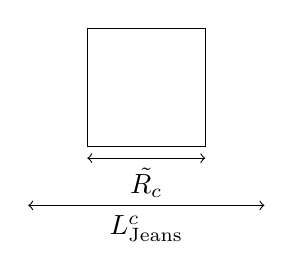
\begin{tikzpicture}[scale=1.5]
			\draw (0, 0) -- (1, 0) -- (1, 1) -- (0, 1) -- (0, 0);
			\draw[<->] (0, -0.1) -- (1, -0.1);
			\draw (0.5, -0.1) node[below] {$\tilde{R_c}$};
			\draw[<->] (-0.5, -0.5) -- (1.5, -0.5);
			\draw (0.5, -0.5) node[below] {$L_\mathrm{Jeans}^c$};
		\end{tikzpicture}
	\end{wrapfigure}
	Vouloir faire une simulation avec un cube interagissant, c'est bien beau, mais un tel objet risque de s'effondrer plutôt vite. Il va nous falloir une condition pour pouvoir le stabiliser.
	Une sphère homogène est stable si sa taille est inférieur à sa longueur de Jeans. Notre critère est donc le suivant:
	\begin{align}
		R_c &\le L_\mathrm{Jeans}^c = \dfrac{\sigma_c^2}{\sqrt{G\rho_c}} \\
		R_c^2 &\leq \dfrac{\sigma_c^2}{G\rho_c} \notag \\
		R_c^2 &\leq \dfrac{\sigma_c^2 R_c^3}{GM_c} \notag \\
		\intertext{Soit $N_c$ le nombre de particules du cube:} \\
		1 &\leq \dfrac{\sigma_c^2R_c}{GN_c m_c} \notag
	\end{align}
	Nous imposons aux particules du cube d'avoir la même masse que celle du Hénon, soit:
	\begin{align*}
		m_c = m_h = m = \dfrac{M_h}{N_h}
	\end{align*}
	où $N_h$ est le nombre de particules du Hénon. Notre critère devient:
	\begin{align}
		1 &\leq \dfrac{\sigma_c^2R_cN_h}{GN_c M_h} \notag \\
		GM_h\dfrac{1}{\sigma_c^2}\dfrac{N_c}{N_h} &\leq R_c \notag
	\end{align}
	en oubliant pas que: $G=1$ et $M_h=1$.
	\begin{align}
		\dfrac{1}{\sigma_c^2} \dfrac{N_c}{N_h} &\leq R_c \label{simu::eq::idee4_jeans}
	\end{align}
	

\subsection{Conditions de la simulation}
	Comme nous cherchons à vérifier notre modèle, nous devons placer le bain à une température
	inférieur à celle que la sphère de Hénon atteint une fois à l'équilibre. Soit $\sigma_h^f$ la
	dispersion de vitesse de la sphère après effondrement, on doit avoir:
	\begin{align}
		\sigma_c &< \sigma_h^f \label{simu::eq::idee4_sig}
	\end{align}

	En parallèle, il serait bon d'éviter que le bain détruise la sphère de Hénon. Il faudrait
	donc avoir:
	\begin{align}
		\rho^f\(R\) \geq \rho_c \label{simu::eq::idee4_dens}
	\end{align}
	où $\rho^f\(R\)$ représente la densité au bord de la sphère, une fois l'équilibre
	atteint.

\subsection{Critères de sélections des paramètres}
	En combinant les équations \ref{simu::eq::idee4_dens}, \ref{simu::eq::idee4_sig} et
	\ref{simu::eq::idee4_jeans}, nous obtenons l'ensemble d'équations suivant:
	\begin{align}
		\begin{cases}
			\dfrac{1}{\sigma_c^2} \dfrac{N_c}{N_h} \leq R_c \\
			\\
			\sigma_c < \sigma_h^f
		\end{cases}
	\end{align}
	%avec $R_h$ le rayon de la sphère une fois l'équilibre atteint, sans le bain.

\subsection{Jeux des paramètres}
	Pour vérifier l'influence du bain, nous devrons jouer sur sa température (sa dispersion de vitesse).
	Mais, nous souhaitons conserver les autres paramètres les moins inchangées possible. Par exemple,
	tel que la simulation est construite, un certains nombres de particules $n_c$ sont directement
	incluse dans le Hénon qui se retrouve alors avec $N_h + n_c$ particules et donc une masse de $M_h + n_c m$.
	De ce fait, pour avoir les simulations les plus similaires possible, nous devons conserver la densité moyenne
	du cube $\rho_c$ constante afin de conserver au mieux $n_c$.

	Voyons comment se comporte notre système:
	\begin{align}
		\rho_c = \dfrac{M_c}{R_c^3} = \dfrac{mN_c}{R_c^3}
	\end{align}
	Nous faisons évoluer notre dispersion de vitesse tel que:
	\begin{align*}
		\sigma_c' = k \sigma_c
	\end{align*}
	en conservant:
	\begin{align}
		\rho_c' = \rho_c \label{simu::eq::idee4_cubedens}
	\end{align}
	Le nouveau rayon s'écrit:
	\begin{align}
		R_c' &= \dfrac{1}{\sigma_c'^2}\dfrac{N_c'}{N_h} = \dfrac{1}{k^2\sigma_c^2}\dfrac{N_c'}{N_h} \notag \\
		\intertext{En utilisant \ref{simu::eq::idee4_cubedens}:}
		\rho_c' &= \rho_c \notag \\
		\dfrac{m N_c}{\(\dfrac{1}{k²\sigma_c²}\dfrac{N_c'}{N_h}\)^3} &= \dfrac{m N_c}{\(\dfrac{1}{\sigma_c²}\dfrac{N_c}{N_h}\)^3} \notag \\
		\dfrac{1}{\dfrac{1}{k^6}N_c'^2} &= \dfrac{1}{N_c^2} \notag \\
		N_c' &= k^3 N_c
	\end{align}
	Ainsi, en augmentant d'un facteur $k$ la dispersion de vitesse, il faut augmenter d'un facteur $k^3$ le nombre de particules dans le cube.

\subsection{Test de stabilité du cube dans ces conditions}
	\begin{figure}
		\begin{center}
			\includegraphics[width=\textwidth]{graphe/dc.png}
			\caption{Carte de l'objet à $t=0$}
			\label{simu::graphe::dccarte0}
		\end{center}
	\end{figure}
	\begin{figure}
		\begin{center}
			\includegraphics[width=\textwidth]{graphe/dc500.png}
			\caption{Carte de l'objet à $t=50$}
			\label{simu::graphe::dccarte50}
		\end{center}
	\end{figure}
	\begin{figure}
			\begin{minipage}[b]{0.40\linewidth}
				\centering \includegraphics[width=\textwidth]{graphe/test_simu_temp.pdf}
				\caption{Température moyenne de l'objet}
				\label{simu::graphe::temp}
			\end{minipage}\hfill
			\begin{minipage}[b]{0.48\linewidth}
				\centering \includegraphics[width=\textwidth]{graphe/test_simu.pdf}
				\caption{Viriel de l'objet}
				\label{simu::graphe::viriel}
			\end{minipage}
	\end{figure}

\subsection{Évolution d'une sphère de Hénon isolée}
	\subsubsection{Évolution dans le vide}
		Des simulations sur l'évolution d'une sphère de Hénon dans le vide on été faîte avec le même
		jeux de paramètres. Ces simulations serviront de référence pour celle avec bain. Toutes ont
		été faîtes jusqu'au temps $t = 50$ dans les unités indiqués section~\ref{simu::sec::unit}.

		\begin{figure}
			\begin{center}
				\includegraphics[width=\textwidth]{graphe/All_parameters.pdf}
				\caption{Évolution dans le temps des paramètres}
				\label{simu::graphe::Parameter}
			\end{center}
		\end{figure}

	\subsection{Effet du nombre de particule}
		Les simulations mentionnées dans le paragraphe précèdent ont été faîtes avec 300 000 et 1 000 000
		de particules. Le graphique~\ref{simu::graphe::densitecomp} compare les profiles de densité volumiques de masse
		à la fin de chacune des simulations.

		\begin{figure}
			\begin{center}
				\includegraphics[width=\textwidth]{graphe/comparison_between_310part.pdf}
				\caption{Comparaison de l'état final entre une simulation de 300 000 particules et une de 1 000 000 de particules.}
				\label{simu::graphe::densitecomp}
			\end{center}
		\end{figure}


